\documentclass[12pt]{article}
\usepackage{amsfonts, epsfig}
\usepackage[authoryear]{natbib}
\usepackage{array}
\usepackage{multirow}
\usepackage{graphicx}
\usepackage{fancyhdr}
\pagestyle{fancy}
\lfoot{\texttt{ematm0067.github.io} / \texttt{ematm0044.github.io}}
\lhead{Introduction to AI - 02.1\_knn - Conor}
\rhead{\thepage}
\cfoot{}

\usepackage{tikz}
\usetikzlibrary{positioning}

\usepackage{ifthen}
\newboolean{nopics}
\setboolean{nopics}{true}


\begin{document}

\section*{$k$-Nearest Neighbours.} 

We will need to think a bit more about the nature of inference, how we
can assess it and how we training algorithms, before we do so, it
might be useful to look at a couple of examples of supervised
learning. We will look at the $k$-nearest neighbours (k-nn) algorithm
first, this algorithm has the virtue of being straight-forward and
easy to understand; it is also, in the language of statistical
modelling, `model free', it does not posit a particular structure for
the data, though, as we will see, it does assume that the distance
measure on the space of data is meaningful. After this we will look at
regression, this make a very strong assumption about the structure of
the data, but turns out to be both surprisingly useful and an
important starting point for thinking about how inference can work. In
short, the k-nn algorithm is useful and, perhaps, prompts us to think
about `representations', how we describe the data in numbers, but the
following topic, regression, is probably more important as an example
of how inference works. Of course, it is good to know about both.

The idea behind k-nn is simple: you have some data
$\{(\textbf{x}_i,y_i)\}$ consisting of input, label pairs. Now, given
a new point $\textbf{x}$ with no label you look at the $k$ nearest
points to $\textbf{x}$ and see what labels they have. You assign
$\textbf{x}$ to whichever label is most common among the
neighbours. This raises the question as to what $k$ is, $k$ is what in
modern parlance, is called a meta-parameter, it is a number you pick
when designing the algorithm; we will discuss the trade-off made in
picking $k$ further and, later, we will discuss a procedure for
selecting the value.

Here is an example; the ducks and rabbits represent the labelled data,
the black arrow points towards an unlabelled data point. Here, $k=8$,
the points inside the circle, of these six are rabbits, so the
unlabelled point would be labelled a rabbit.
\begin{center}

\begin{tikzpicture}[scale=1.0]
    % Draw axes
    \draw[thick,->] (-5,0) -- (5,0) node[right] {};
    \draw[thick,->] (0,-5) -- (0,5) node[above] {};


%rabbits
    \foreach \x/\y in {-4/2, -2/1, -1/3, 0/5, 1/-2.5, 2/3, 4/4, 4.5/5}
        \node at (\x,\y) {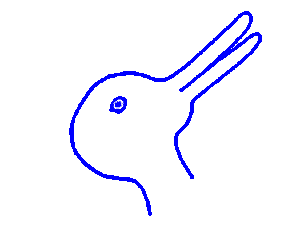
\includegraphics[width=1cm]{rabbit.png}};

        %ducks
    \foreach \x/\y in {-4/-1, -3/-4, -2/4, -1/-4, 1/-1, 2/-2.1, 3.1/2, 4/-1.1, 4.5/-2}
        \node at (\x,\y) {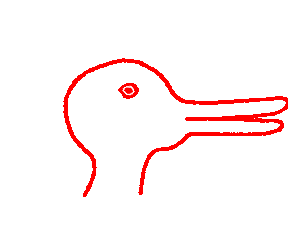
\includegraphics[width=1cm]{duck.png}};

% Additional rabbits
        \foreach \x/\y in {-3/2.5, -2.7/4.1, -1.5/-0.75, 0.75/4.2, 1.5/1.2, 3/3.5, 3.5/-4, 4/3}
        \node at (\x,\y) {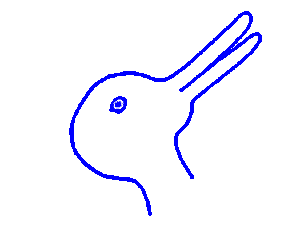
\includegraphics[width=1cm]{rabbit.png}};

    % Additional ducks
    \foreach \x/\y in {-3.5/-2, -2.5/-3, -2/-3.5, -1.5/-2, 0.5/2, 1.5/-1.5, 2.5/-2.5, 3.4/1.1, 4.5/-3}
        \node at (\x,\y) {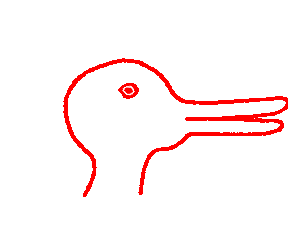
\includegraphics[width=1cm]{duck.png}};

\node at (-2,2) {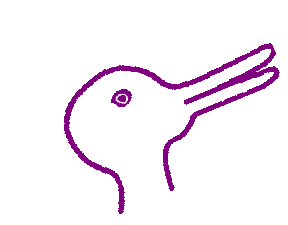
\includegraphics[width=1cm]{what.png}};        

\draw[black, thick] (-2,2) circle (3.25cm); % Adjust the radius as needed

\draw[->, >=stealth, line width=1mm, black] (-4,1) -- (-2.5,1.75); 
\end{tikzpicture}
\end{center}

Obviously the notion of $k$-nearest neighbours relies on a metric on
the space the data are in: the obvious thing is to just take the Euclidean distance:
\begin{equation}
  d_{ij}=\|\mathbf{x}_i-\mathbf{x}_j\|
\end{equation}
but this does reply on the co\"{o}rdinates representing properties of
the data relevant to the labelling. If the co\"{o}rdinates have
nothing to do with the labelling the approach will not work:
\begin{center}
\begin{tikzpicture}[scale=1.0]
    % Draw axes
    \draw[thick,->] (-5,0) -- (5,0) node[right] {};
    \draw[thick,->] (0,-5) -- (0,5) node[above] {};

    % Rabbits
    \foreach \x/\y in {-2.5/-3,-2/4,  2.5/-2.5,2/-2.1, -1.5/-0.75, 4/3 , 1.5/1.2, -4/2, 0.75/4.2, 4.5/5, 3/3.5, 1/-2.5, -1/-4 ,  -4/-1, 3.4/1.1} 
        \node at (\x,\y) {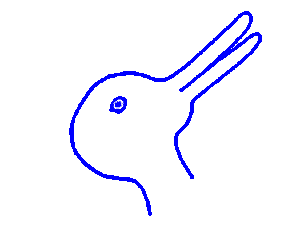
\includegraphics[width=1cm]{rabbit.png}};


        
    % Ducks
    \foreach \x/\y in {0/5, 2/3,  -2/-3.5,1/-1, -3/-4, -1.5/-2, 3.1/2, -3/2.5, 3.5/-4,  -1/3, -2.7/4.1, 0.5/2, -3.5/-2, 4/-1.1, 1.5/-1.5, 4.5/-3,-2/1, 4/4}
    \node at (\x,\y) {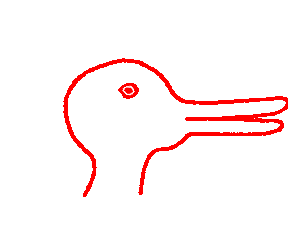
\includegraphics[width=1cm]{duck.png}};

    % "What" image
    \node at (-2,2) {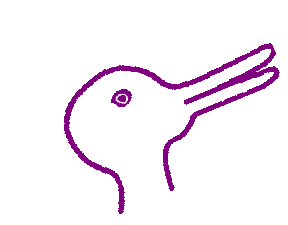
\includegraphics[width=1cm]{what.png}};        

    % Circle around "what.png"
    \draw[black, thick] (-2,2) circle (3.25cm); % Adjust the radius as needed

    % Arrow pointing at "what.png"
    \draw[->, >=stealth, line width=1mm, black] (-4,1) -- (-2.5,1.75); 
\end{tikzpicture}
\end{center}
In this case the unlabelled point will be labelled as a duck, but
looking at the mix of datapoints it is not clear that that is useful,
the location of each point has little to do with its label. This
problem is one of representation, the datapoints are being represented
by the co\"{o}rdinates, but these may not represent the label in a
useful way. In many algorithms some part of the computations relates
to finding a good representation, which may involve a mapping of the
original co\"{o}rdinate.

Conversely a strength of k-nn is that it does not assume the location
represents the label in any particular way, it just assumes that
points with a particular label a likely to be near other points with
that label, this example shows data where the division between ducks
and rabbits does not lie on a single line:
\begin{center}
\begin{tikzpicture}[scale=1.0]
    % Draw axes
    \draw[thick,->] (-5,0) -- (5,0) node[right] {};
    \draw[thick,->] (0,-5) -- (0,5) node[above] {};

    % Rabbits
    \foreach \x/\y in {0/5, 2/3,-2.5/-3,   -2/-3.5, -1.5/-0.75, 4/3 , 1.5/1.2, 0.75/4.2, 4.5/5, 3/3.5, 1/-2.5, -1/-4 ,  -4/-1, 3.4/1.1, 0.5/2, -3.5/-2, 4/4} 
        \node at (\x,\y) {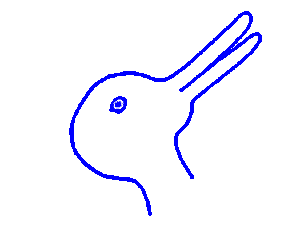
\includegraphics[width=1cm]{rabbit.png}};


        
    % Ducks
        \foreach \x/\y in { 2.5/-2.5,2/-2.1
          ,-2/4,1/-1, -3/-4, -1.5/-2, 3.1/2, -3/2.5, 3.5/-4,  -1/3, -4/2, -2.7/4.1, 4/-1.1, 1.5/-1.5, 4.5/-3,-2/1}
    \node at (\x,\y) {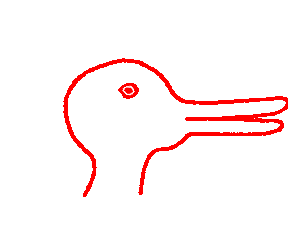
\includegraphics[width=1cm]{duck.png}};

    % "What" image
    \node at (-2,2) {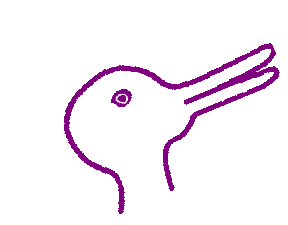
\includegraphics[width=1cm]{what.png}};        

    % Circle around "what.png"
    \draw[black, thick] (-2,2) circle (3.25cm); % Adjust the radius as needed

    % Arrow pointing at "what.png"
    \draw[->, >=stealth, line width=1mm, black] (-4,1) -- (-2.5,1.75); 
\end{tikzpicture}
\end{center}
Nonetheless the k-nn approach is useful here. In passing, it should
also be noted that the approach does not rely on the distance in a
detailed way, it uses it only to calculate proximity. Indeed you might
expect the approach to work well even if the space of data does not
have co\"{o}rdinates but does have a way of calculating distance, as
happens, for example, with time series.

Finally there is the vexing issue of how to pick $k$. $k$ is a sort of
`smoothing parameter' and as always with smoothing parameters, if it
is too small it doesn't smooth and if it is too big it smooths away
the stuff you are actually interested in. A very contrived
illustration is given here:
\begin{center}
\begin{tikzpicture}[scale=1.0]
    % Draw axes
    \draw[thick,->] (-5,0) -- (5,0) node[right] {};
    \draw[thick,->] (0,-5) -- (0,5) node[above] {};

    % Rabbits
    \foreach \x/\y in {2.5/-3, -1.5/1.5,   1.5/-0.75,1.5/-0.25, 0.2/-.5, 2/-2, 0.75/-0.75, 1/-2.5, 1/-4 ,  4/-1} 
        \node at (\x,\y) {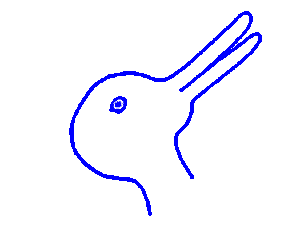
\includegraphics[width=1cm]{rabbit.png}};


        
    % Ducks
        \foreach \x/\y in {-2.5/0.75, -3/2.5,-2/2.8, -3/4, -4/4, -2.5/1.8, 2/-3.5}
    \node at (\x,\y) {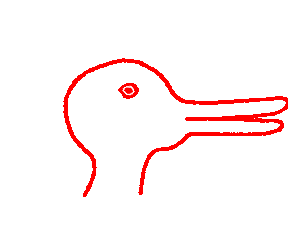
\includegraphics[width=1cm]{duck.png}};

    % "What" image
    \node at (-1,1) {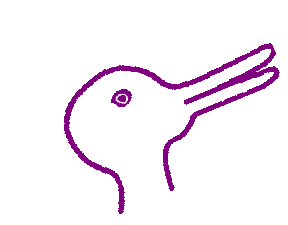
\includegraphics[width=1cm]{what.png}};        

    % Circle around "what.png"
    \draw[black, thick, dashed] (-1,1) circle (3.25cm); % Adjust the radius as needed
    \draw[black, thick] (-1,1) circle (2.25cm); % Adjust the radius as needed
    \draw[black, thick, dotted] (-1,1) circle (1.25cm); % Adjust the radius as needed

    % Arrow pointing at "what.png"
    \draw[->, >=stealth, line width=1mm, black] (-3,0) -- (-1.5,0.75); 
\end{tikzpicture}
\end{center}
Here, it is clear there is a rabbit cluster and a duck cluster; there
is a duck in the rabbit cluster and a rabbit in the duck cluster; this
represents the possibility of mislabelling or other noise. Now if
$k=5$, corresponding to the cicle with a solid boundary, the
unlabelled point is labelled duck, which is probably correct; if $k=1$
this is a $k$ value much more vulnerable to noise and, indeed here it
would result in the unlabelled point being labelled rabbit, similarly,
if $k=9$, corresponding to the dashed circle the neighbourhood is
larger than the clustering structure of the label and, again, the
unlabelled point would be labelled rabbit.

In the next section we will look at cross-validation, which gives a
strategy for picking $k$. 

\section*{Summary}
In k-nearest neighbours, often called knn or k-nn, you look at the
$k$-nearest points to an unlabelled point and give it the label
corresponding to the most common label in the group. It is
straight-forward and model free, but does assume the distance you use
in `nearest' is meaningful. It also relies on a choice of $k$, if $k$
is too small then the labelling is vulnerable to noise, if it is too
big the labelling might miss the structure of the data.

\end{document}

